\chapter{Implementation}
\label{sec:implementation}

We have implemented \Backpack{} in GHC 8.2 and cabal-install 2.0.  In
this chapter, we describe some aspects of our implementation.

\section{Opaque unit identifiers}
\label{sec:opaque-uid}

\Uid{}s are abstract syntax trees which are passed around throughout
both GHC and Cabal.  The downside is that instantiated \uid{}s
can be quite large (in part because \cid{}s allocated by the
package manager can be quite large, as they must record information
about how dependency resolution was performed for the library).

Fortunately, in some cases, the structure of a \uid{} is not necessary;
for example, when a unit identifier has no module holes, it is
invariant under substitution.  A useful optimization in this case
is to represent the structure opaquely with a \emph{definite unit
identifiers}.

GHC and Cabal implement this optimization, changing the
abstract structure of a \uid{} to look like this:

\[
\begin{array}{rcll}
  \mathbb{P} &&& \text{Definite \uid{}} \\
  \UP &::=& \icid{\Up}{S} & \text{\Uid} \\
      & | & \mathbb{P} \\
\end{array}
\]

\noindent
Notice that definite \uid{}s occur recursively: the intent is that a
definite \uid{} be allocated for a library when it is fully instantiated
and compiled.  Thus, a definite \uid{} always corresponds to a \uid{}
whose module substitution refers all to definite \uid{}s (since those
libraries had to be compiled first, before this one could be compiled!)
When compiling a fully instantiated library, the only \uid{}s which the
compiler needs to interact with are definite \uid{}s, meaning that we
only have to pay the cost of a full \uid{} when typechecking uninstantiated
libraries.

Definite \uid{}s are purely an implementation mechanism; if a definite
\uid{} and a normal \uid{} are compared, the comparison must be done
up to unfoldings of the definite \uid{}, as seen below (definite \uid{}s
highlighted in blue):

\begin{figure}[H]
\center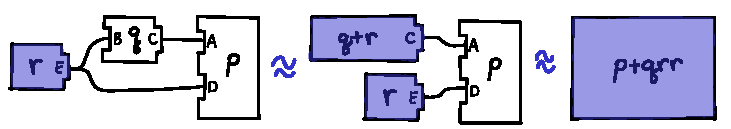
\includegraphics{figures/unit-identifier-improvement.pdf}
\end{figure}

\section{Modifications to GHC}

As far as possible, the typechecking rules described in
Section~\ref{sec:compiler} are a faithful rendering of our
actual implementation of \Backpack{} in GHC\@: each rule
is in direct correspondence to some functionality in
GHC\@.  To help readers interested in perusing \Backpack{} in GHC's
source code, Table~\ref{table:semantic-objs} gives a correspondence
between a semantic object and its corresponding type name in GHC\@;
similarly, Table~\ref{table:judgments} gives a correspondence between
our judgments and their implementations in GHC\@.

In our primary \Backpack{} patch (not counting subsequent bugfix
patches, as well as some preliminary support for signatures that we had
committed previously), we modified 40 files in the compiler (out of 513
source files in the \verb|compiler| directory), adding 4375 lines and
deleting 588 lines.  In this respect, we think that our \Backpack{}
patch is quite well-contained: by in large, we were able to implement
\Backpack{} with minimal changes to the renamer and typechecker.
However, there is one major complication, related to GHC's lack
of \emph{symbol tables}, which we discuss in the next section.

\begin{table}
\centering
\begin{tabular}{llllll}
Semantic entity & & GHC type & Defined In \\
\midrule
Module name & $m$ & \verb|ModuleName| & \verb|Module| \\
Component identifier & $p$ & \verb|ComponentId| & \verb|Module| \\
Module identifier & $M$ & \verb|Module| & \verb|Module| \\
Unit identifier & $P$ & \verb|UnitId| & \verb|Module| \\
Module type & $T$ & \verb|ModIface|/\verb|ModDetails| & \verb|HscTypes| \\
Type declaration & \I{decl} & \verb|IfaceDecl|/\verb|TyThing| & \verb|IfaceSyn|/\verb|TyCoRep| \\
Class instance & \I{inst} & \verb|IfaceClsInst|/\verb|ClsInst| & \verb|IfaceSyn|/\verb|InstEnv| \\
Family instance & \I{inst} & \verb|IfaceFamInst|/\verb|FamInst| & \verb|IfaceSyn|/\verb|FamInstEnv| \\
Occurrence name & $n$ & \verb|OccName| & \verb|OccName| \\
Original name & $N$ & \verb|Name| & \verb|Name| \\
Name substitution & $\USn$ & \verb|NameShape| & \verb|NameShape| \\
Haskell type/kind & $\tau, \kappa$ & \verb|IfaceType|/\verb|Type| & \verb|IfaceType|/\verb|TyCoRep| \\
External component type context & $\Gamma$ & \verb|ExternalPackageState| & \verb|HscTypes| \\
Local type context & $\Delta$ & \verb|HomePackageTable| & \verb|HscTypes| \\
\end{tabular}
\caption{Mapping from semantic objects in this thesis (Figure~\ref{fig:lcomponents} and Figure~\ref{fig:semantic-objects}) to their definitions
in GHC\@.  In some cases, a semantic object maps to two types in GHC\@; see Section~\ref{sec:no-symbol-tables} for details.}
\label{table:semantic-objs}
\end{table}

\begin{table}
\centering
\begin{tabular}{llll}
Figure & Judgment & GHC Function & Defined In \\
\midrule

Fig.~\ref{typing:haskell} & Module/signature typechecking & \verb|tcRnModule| & \verb|TcRnDriver| \\
& Type/kind equality & \verb|eqType| & \verb|Type| \\
& Instance resolution & \verb|check_inst| & \verb|TcBackpack| \\

Fig.~\ref{typing:main} & Top-level typing & \verb|load| & \verb|GhcMake| \\
& \quad\textsf{exposes} & \verb|applyPackageFlag| & \verb|Packages| \\
& \quad\textsf{inherits} & \verb|collectHoles| & \verb|Packages| \\
& Declaration typing & \verb|hscTypecheck| & \verb|HscMain| \\
& Dependency typing & \verb|tcRnCheckUnitId| & \verb|TcBackpack| \\
& Declaration sequencing & \verb|upsweep| & \verb|GhcMake| \\

Fig.~\ref{typing:lookup} & Original name type lookup & \verb|importDecl| & \verb|LoadIface| \\
& Module type lookup & \verb|loadInterface| & \verb|LoadIface| \\
& Substitution & \verb|rnModIface| & \verb|RnModIface| \\
& Name substitution & \verb|rnIfaceGlobal| & \verb|RnModIface| \\
%& Orphan substitution & (implicit) & \\

Fig.~\ref{typing:merging} & Signature type merging & \verb|tcRnMergeSignatures| & \verb|TcBackpack| \\
& Export list merging & \verb|extendNameShape| & \verb|NameShape| \\
& Declaration list merging & \verb|mergeIfaceDecls| & \verb|TcIface| \\

Fig.~\ref{typing:top-subtyping} & Module subtyping & \verb|checkImplements| & \verb|TcBackpack| \\

Fig.~\ref{typing:subtyping} & Declaration subtyping & \verb|checkBootDecl| & \verb|TcRnDriver| \\
& Declaration pre-subtyping & \verb|checkBootTyCon| & \verb|TcRnDriver| \\
\end{tabular}
\caption{Mapping from typing judgments to implementations in GHC.}
\label{table:judgments}
\end{table}


\subsection{No symbol tables}
\label{sec:no-symbol-tables}

The most important aspect of the implementation not captured by
the rules in Section~\ref{sec:compiler} is GHC's lack of traditional
symbol tables.
Traditionally, compilers have one or more data structures known as
\emph{symbol tables}, which are mappings from symbols to information
about the symbol: abstractly, the symbol table is represented by
the \emph{context} in which typechecking takes place.
Rather than look up information on symbols in a
context, GHC records all of the information about a symbol in
the symbol itself, forming an immutable cyclic data structure of
all symbols known to GHC\@.

For example, here are
some data types for the graph representation from GHC (simplified
and abbreviated):

\begin{lstlisting}
    data Type  = TyConApp TyCon [Type]  | ...
    data TyCon = SynonymTyCon Name Type | ...
    data ModDetails = ModDetails [TyCon] ...
\end{lstlisting}
%
A type may be an application of a type constructor to some arguments, in which
case it contains a type constructor \verb|TyCon|.  A type constructor
can be a type synonym, in which case it contains the type it expands
to.  A module \verb|ModDetails| consists of a list of type constructors
and other entities that are defined in it.  The ``graph'' is the graph of
heap objects which represent these data types.

This graph is very convenient to work with in a purely functional
language like Haskell, since queries can be answered by a direct field
access rather than a lookup in a symbol table.  For example, type
equality can be defined as a pure function \verb|Type -> Type -> Bool|
even in the presence of type synonyms, since the \verb|SynonymTyCon|
always carries along the expanded version of the synonym to compare
against.

On disk, GHC must serialize these direct references to indirect references
by names:

\begin{lstlisting}
    data IfaceType = IfaceTyConApp Name [IfaceType] | ...
    data IfaceDecl = IfaceSynonym OccName IfaceType | ...
    data ModIface = ModIface [IfaceDecl] ...
\end{lstlisting}

\noindent
Unlike the graph representation, the type constructor application
doesn't embed the definition of the type constructor---instead,
it records only a \verb|Name| reference to the constructor. To find out
more information about the type constructor, you would have to lookup
the \verb|IfaceDecl| from the appropriate symbol table; e.g., a module
local declaration would be found in the \verb|IfaceDecl| list in
\verb|ModIface|.

GHC uses a technique called tying the knot
to construct the graph representation from the interface
representation: any time we encounter a \verb|Name|, GHC instead
allocates a thunk to lookup the appropriate declaration later,
once all of the entities have been added to the environment;
this is referred to as ``typechecking'' the interface.

\paragraph{Consequences for \Backpack{}}
In Section~\ref{sec:overview-compiler}, we informally described
types as graphs, with original names pointing to the corresponding
declaration.  In fact, this is an accurate representation of how
these operations are implemented in GHC\@!

One downside of the immutable graph representation is that it is
difficult to modify after the fact: in general, the only way to update
it is to rebuild the graph from scratch.  Modifications of this kind
frequently occur in \Backpack{}: for example, applying a name
substitution will change how the graph is wired.

To handle this, our implementation does most operations in two
phases:

\begin{itemize}
    \item We first perform any operations which would
    mutate the graph on the \emph{interface representation}.
    These operations includes both module and name substitutions, as well
    as signature merging.
    \item Then, we generate the \emph{graph representation} from
    the resulting interface representation, and then perform any
    operations which require consulting the context.  These
    operations include subtyping, which test equality on types
    and require the context.
\end{itemize}
%
Module type lookup is a good example of this two phase process: to
perform module type lookup, we first read in the un-substituted
\verb|ModIface| from the file system, apply the substitution according
to the substitution in the module identity, and \emph{then} typecheck
the interface into the graph representation for using during type
checking.

A more subtle example of this process occurs when performing
signature merging.  When we merge signatures, we eventually need
to check that the merged signature is a subtype of each of the
input signatures, with the \emph{merged} signature in the context.
This means that to perform this subtyping test, GHC first typechecks
each of the input \verb|ModIface|s for the signatures, wiring any
local \verb|Name|s to point to the merged signature, and then performs
the subtyping tests on the resulting graph.  In other words, the
informal description of signature merging in Section~\ref{sec:signature-merging}
is actually quite close to what actually occurs in GHC proper!

\subsection{Miscellaneous differences}

There are a number of smaller differences between our formalization
and GHC's representation.

\begin{itemize}
    \item In our formulation of GHC Haskell's semantic objects, an
    instance directly records the type representing the constraint that
    the instance fills.  In GHC Haskell, an instance instead contains a
    reference to a \emph{dictionary function}, which is just a type of
    term declaration that is never exported.  The two presentations are
    equivalent, but embedding the dictionary function in the instance
    makes it easier to specify the rules instance checking (indeed,
    refactoring GHC to adopt this representation would substantially
    simplify some aspects of the implementation).  Similarly,
    closed family instances are associated with a coercion axiom, but in
    our presentation they are embedded in \I{tfinfo}; because coercion axioms
    are always associated with another declaration, we omit them from the
    production $\Uty$.

    \item We simplified export specifications to just be a list of
    names, rather than names with children (which allows GHC to support
    import declarations like \verb|import Prelude (Eq(..))|).  We've
    implemented an extension to handle children as per Haskell'98; the
    tricky thing is handling the semantics of an export of a bare
    record selector (without the type it is bundled with):

    \begin{lstlisting}
        module A where
            data T = MkT { f :: Int }
        module B(f) where
            import A
        module C(T(..)) where
            import A (T)
            import B (f)
    \end{lstlisting}

    Haskell'98 specifies that \verb|T(..)| selects both \verb|T| and \verb|f|
    for export: a record selector always ``remembers'' what type is its
    parent.  In Haskell'98, a record selector or data constructor
    always comes from the same module as the parent, so when
    we apply a name substitution to \verb|f|, we can infer the new name of
    the parent with directly from the substituted name.

    There are two more features in GHC Haskell which affect export lists:
    \begin{itemize}

        \item Bundled pattern synonyms\footnote{\url{https://ghc.haskell.org/trac/ghc/wiki/PatternSynonyms/AssociatingSynonyms}} make it possible to declare a pattern synonym
            to be a child of a type: in this case, the child of a type may
            be defined in a different module than the type itself.
            \Backpack{} does not support pattern synonyms, so it's
            not possible to have nontrivial bundling between an abstract
            pattern synonym or abstract type in a signature file, but if it
            were to support pattern synonyms this interaction would need to
            be worked out.

        \item Duplicate record fields\footnote{\url{https://ghc.haskell.org/trac/ghc/wiki/Records/OverloadedRecordFields/DuplicateRecordFields}} augment
            every export with a set of associated ``field labels'', which are
            allowed to overlap with other field labels that are in scope.
            These are handled similarly to exported children.
        \end{itemize}

    \item In our formalization, the list of transitive orphan-defining
        modules includes the module itself; GHC stores this separately
        in another flag in the interface file.

    \item In the abstract grammar for module identifiers ($M$) and original
        names ($N$), we have separate cases module holes and name
        holes.  In GHC, we avoid defining an extra constructor
        by instead defining a special unit identifier \cidl{hole}, and saying
        that a module hole $\hv{m}$ is represented as \Mod{\cidl{hole}}{m};
        similarly, a name hole  \nhv{m.n} is represented as $\Mod{\cidl{hole}}{m}.n$.

        Internally representing the holes this way was expedient as it
        allowed us to avoid having to add a lot of new pattern matches
        to GHC, but the tradeoff is that we have to be careful about how
        we go about performing substitutions: for example, we must not apply
        a module substitution on the module identifier of an original name,
        if its top level module identity is a hole module.

    \item Modifications to GHC's \verb|UnitId| data type to support module
        substitutions.  We try to keep \uid{}s represented as plain
        strings as much as possible; see Section~\ref{sec:opaque-uid} for
        more details.

    \item We applied a slight optimization to dependency type-checking in GHC\@:
        rather than defer all dependency type checking to the
        very end of compilation, we incrementally check dependencies for well-typedness
        as we finish typechecking all the local signatures for the dependency's
        requirements.

\end{itemize}
%


\section{Modifications to Cabal}

Our implementation of \Backpack{} in Cabal also closely follows the description
from Section~\ref{sec:overview}.  There are three primary phases in our
implementation:

\begin{enumerate}
    \item Given the original Cabal source file, we elaborate each
    component it defines into \emph{configured component},
    for which we've resolved all source-level dependencies
    (e.g., entries in \verb|build-depends|) to the specific
    \cid{}s representing them, incorporating in the information
    we learned from dependency resolution.

    \item We then perform mixin linking, producing \emph{linked component}
    where every \cid{} has been further elaborated into a \uid{}
    representing exactly how the dependencies are instantiated.
    Mixin linking is essentially a direct implementation of the
    description we gave in Section~\ref{sec:mix-in}.

    \item Finally, we zip through all fully instantiated components
    and recursively instantiate their dependencies, producing one or
    more \emph{ready components} per source component.  Each ready
    component represents a component plus a complete instantiation,
    and represents a separate compilation we will do (with full
    knowledge of how the dependencies are instantiated).
\end{enumerate}
%
We did need to apply one nontrivial architectural change to Cabal.
Previously, Cabal was organized into two parts:

\begin{itemize}
    \item The \emph{build system}, e.g., Cabal, which is responsible for
    building a single package, and

    \item The \emph{package manager}, e.g., cabal-install, which is
    responsible for building multiple packages.
\end{itemize}
%
A single package may itself contain multiple components (beyond the library,
there may be test suites, executables, etc.). Historically, a package manager
invoked Cabal the build system once to build all the components at once.

This architecture causes problems for \Backpack, where a library may need
to be built multiple times because it was reinstantiated: in this case, we really want to
rebuild just the library (and not the executables, test suites, etc.).
So, instead, we added a new mode to the Cabal build system to operate
on a per-component basis:\footnote{https://github.com/ghc-proposals/ghc-proposals/pull/4}
the \emph{build system} builds a single \emph{component}, and
the \emph{package manager} builds multiple components.  For \Backpack{} to be
supported by Stack (an alternative package manager implementation), we'll have
to apply this architectural change as well.
